\chapter{FUNDAMENTO TEÓRICO}
\markboth{CAPÍTULO \thechapter: FUNDAMENTO TEÓRICO}{}
\section{ANTECEDENTES DE INVESTIGACIÓN}

\subsection{Revisión de métodos}
\subsubsection{Antecedente 1}

\lipsum[1]

\begin{figure}[H]
  \centering
  \caption{Diseño del sistema del artículo 1}
  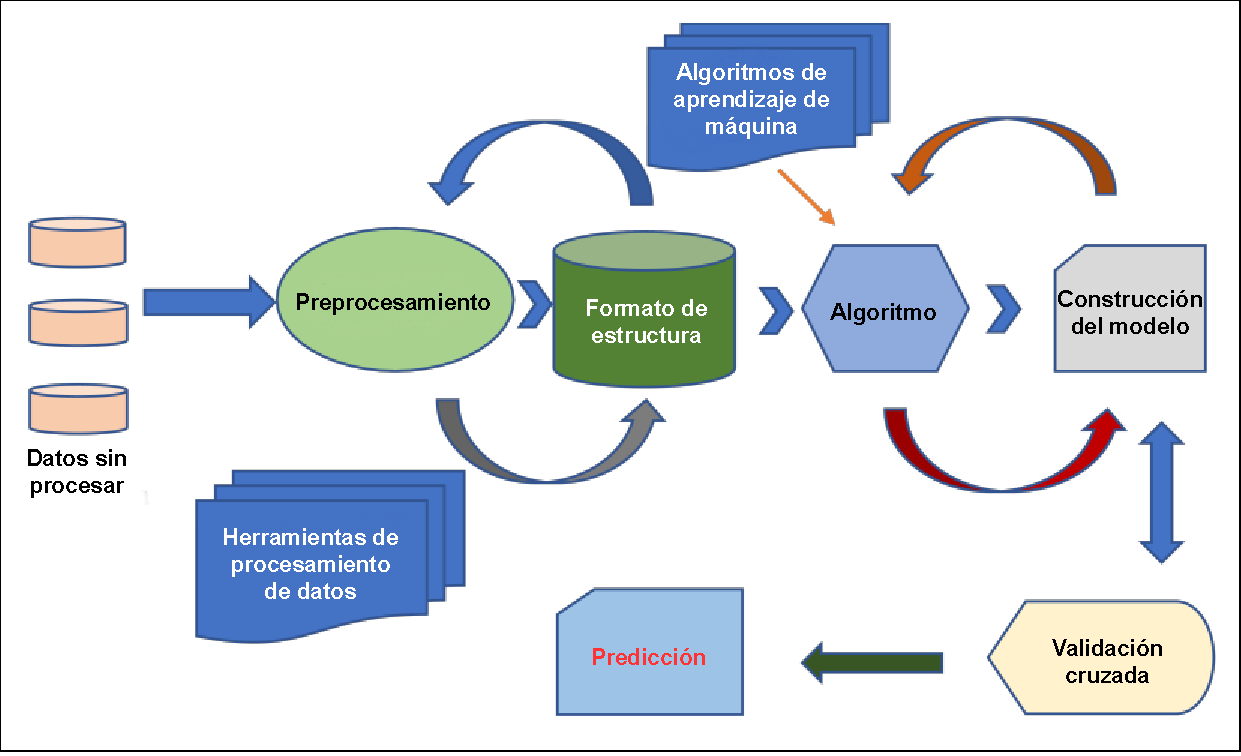
\includegraphics[width=0.8\textwidth]{E_IMAGENES/1_Capitulo2/1-research-background/Paper_1_1.pdf}
  \caption*{Fuente: \citet{9276955}}
  \label{fig:Imagen_1}
\end{figure}

\lipsum[2]

\begin{table}[H]
  \centering
  \caption{Resultados del artículo 1}
  \begin{tabular}{cccc} 
  \hline
  \textbf{Modelo}          & \textbf{Exactitud} & \textbf{Precisión} & \textbf{Sensibilidad}  \\ 
  \hline
  Árbol de
    decisión      & 0.96               & 0.75               & 0.7                    \\ 
  \hline
  Bosque
    aleatorio       & 0.95               & 1                  & 0.17                   \\ 
  \hline
  Naive Bayes
    Gaussiano  & 0.99               & 1                  & 0.88                   \\ 
  \hline
  K vecinos más
    cercanos & 0.93               & 0.44               & 0.23                   \\
  \hline
  \end{tabular}
  \caption*{Fuente: \citet{9276955}}
  \label{tab:Paper_1_3}
\end{table}

\subsubsection{Antecedente 2}

\lipsum[2]

\begin{figure}[H]
  \centering
  \caption{Resultados del enfoque global del artículo 2}
  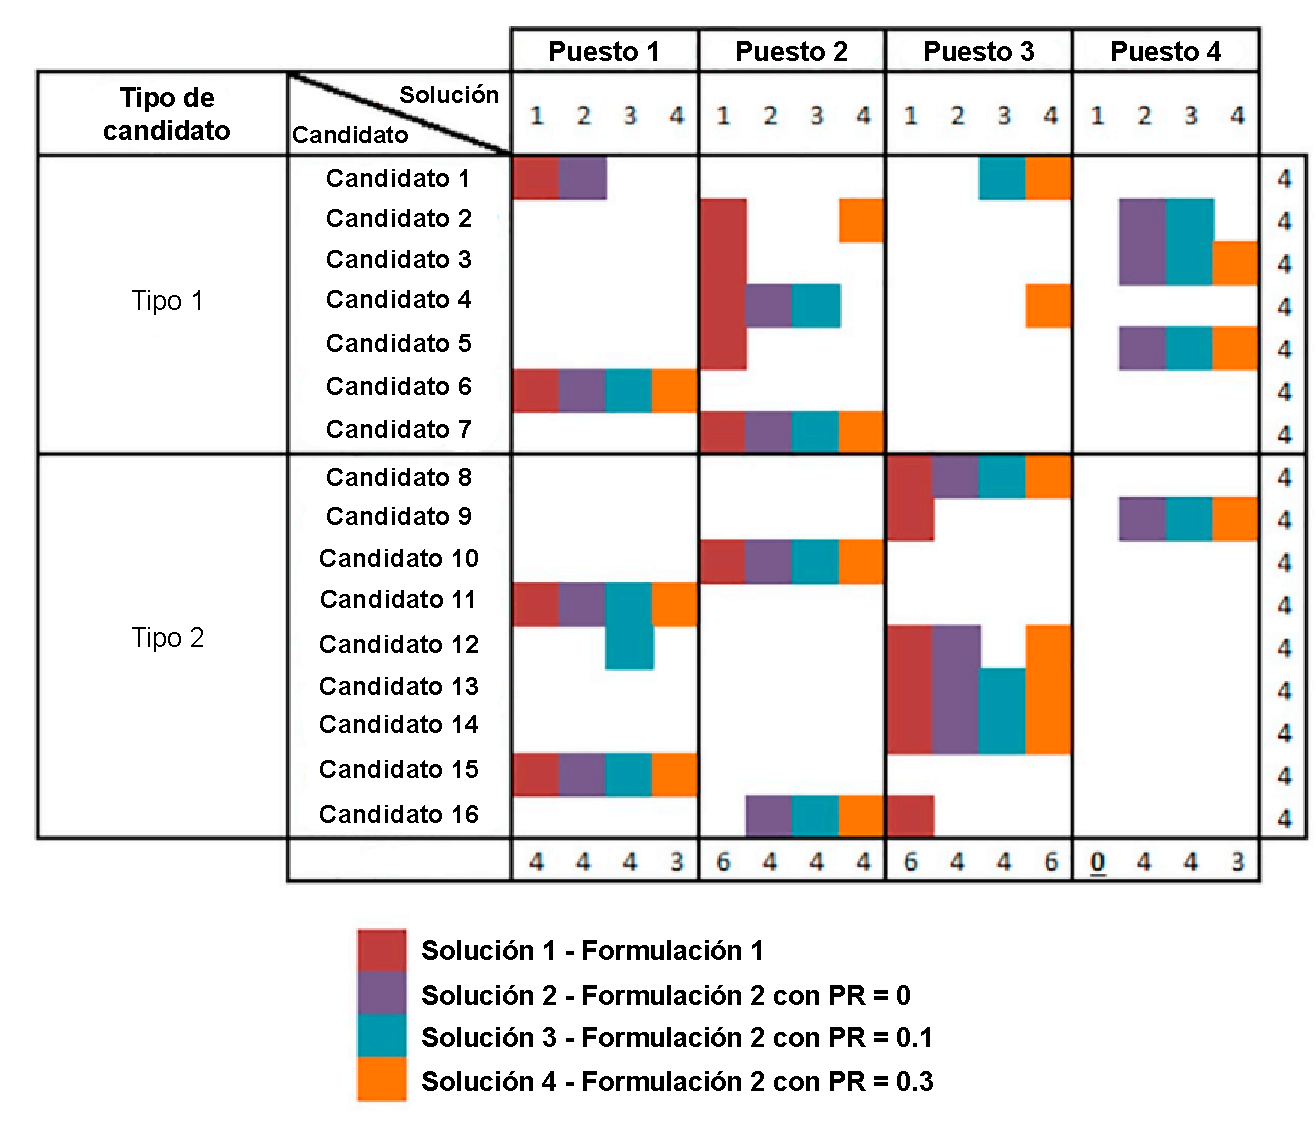
\includegraphics[width=1.0\textwidth]{E_IMAGENES/1_Capitulo2/1-research-background/Paper_2_2.pdf}
  \caption*{Fuente: \citet{PESSACH2020113290}}
  \label{fig:Paper_2_2}
\end{figure}

\subsubsection{Antecedente 3}

\lipsum[3]

\begin{table}[H]
  \centering
  \caption{Resultados del artículo 3}
  \resizebox{\columnwidth}{!}{
    \begin{tabular}{ccccc} 
    \hline
    \begin{tabular}[c]{@{}c@{}}\textbf{Tamaño de la muestra}\end{tabular} & \begin{tabular}[c]{@{}c@{}}\textbf{Exactitud (\%)}\end{tabular} & \begin{tabular}[c]{@{}c@{}}\textbf{Especificidad (\%)}\end{tabular} & \begin{tabular}[c]{@{}c@{}}\textbf{Sensibilidad (\%)}\end{tabular} & \begin{tabular}[c]{@{}c@{}}\textbf{Robustez (\%)}\end{tabular}  \\ 
    \hline
    100                                                                              & 96.2                    & 94.2                        & 94.8                       & 94.5                    \\ 
    \hline
    200                                                                              & 95.4                    & 95.6                        & 95.2                       & 95.4                    \\ 
    \hline
    300                                                                              & 94.8                    & 93.6                        & 93.9                       & 93.7                    \\ 
    \hline
    400                                                                              & 95.8                    & 93.8                        & 95.1                       & 94.6                    \\ 
    \hline
    500                                                                              & 93.2                    & 95.2                        & 92.9                       & 94.3                    \\ 
    \hline
    600                                                                              & 86.2                    & 85.6                        & 86.6                       & 86.2                    \\ 
    \hline
    700                                                                              & 92.8                    & 94.4                        & 94.6                       & 94.5                    \\ 
    \hline
    800                                                                              & 94.4                    & 95.2                        & 94.8                       & 95.1                    \\ 
    \hline
    900                                                                              & 93.8                    & 94.6                        & 95.1                       & 94.8                    \\ 
    \hline
    1000                                                                             & 88.5                    & 87.8                        & 85.6                       & 86.3                    \\ 
    \hline
    1100                                                                             & 94.7                    & 96.2                        & 93.8                       & 94.2                    \\ 
    \hline
    1200                                                                             & 96.1                    & 95.2                        & 93.2                       & 94.5                    \\ 
    \hline
    \textbf{1300}                                                                             & \textbf{96.96}                   & \textbf{96.38}                       & \textbf{96.02}                      & \textbf{96.26}                   \\
    \hline
    \end{tabular}
  }
  \caption*{Fuente: \citet{StackedKNN}}
  \label{tab:Paper_3_4}
\end{table}

\subsubsection{Antecedente 4}

\lipsum[4]

\begin{figure}[H]
  \centering
  \caption{Metodología a usar del artículo 4}
  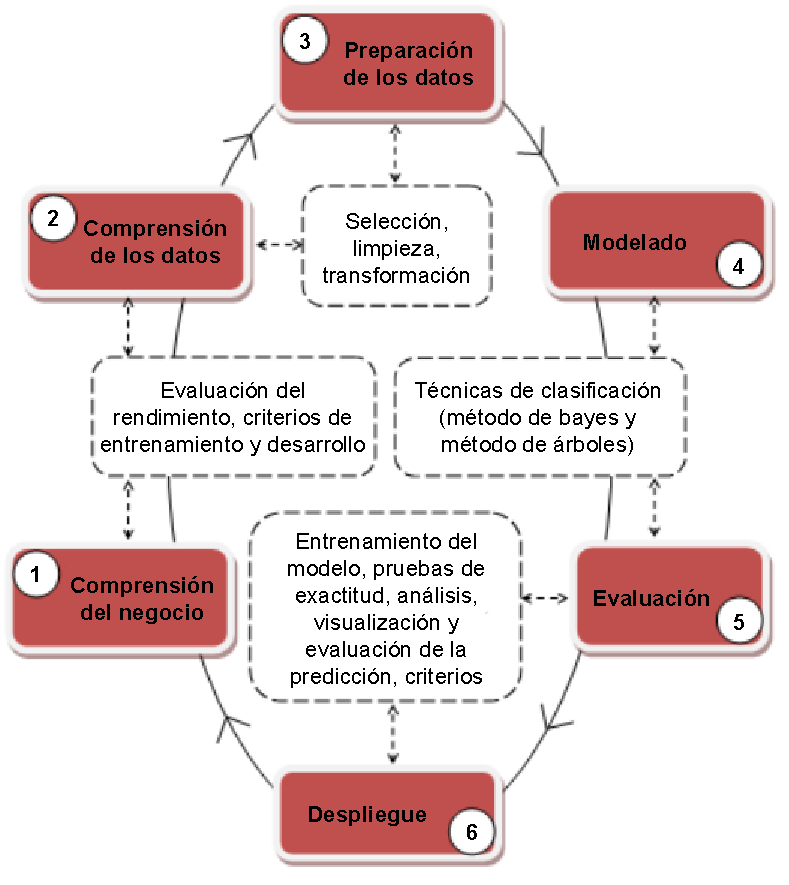
\includegraphics[width=0.8\textwidth]{E_IMAGENES/1_Capitulo2/1-research-background/Paper_4_1.pdf}
  \caption*{Fuente: \citet{arxiv2013}}
  \label{fig:Paper_4_1}
\end{figure}

\subsubsection{Antecedente 5}

\citet{IJET11738} sostiene que, por un lado, los estudiantes deben prepararse desde etapas tempranas de su formación para adaptarse a la vida laboral y evaluar constantemente su desempeño.

Y, por otro lado, los reclutadores primero evalúan a los candidatos en diferentes parámetros y luego eligen en que puesto de trabajo deben mantener al candidato según su desempeño, y en base al aporte que puede realizar a la organización \citep{IJET11738}.

\subsection{Evaluación comparativa}

\lipsum[6]

\subsection{Usos alternativos o aplicaciones varias}

\lipsum[7]

\subsection{Software o sistemas existentes}

\lipsum[8]

\section{BASES TEÓRICAS}

\subsection{Variable dependiente: Nombre de la VD}

\lipsum[9]

\subsection{Variable independiente: Nombre de la VI}

\lipsum[10]
